The CMS detector was designed with two primary physics goals in mind.
First, to study the properties of the Higgs boson; in particular, the nature of electroweak symmetry breaking for which the Higgs mechanism is responsible\footnote{Note that during the design of the CMS detector, the Higgs boson was theorized to exist but had not yet been discovered.}.
Second, to reveal signs of physics beyond the Standard Model which might be present at the TeV scale.
This section discusses technical design aspects of the CMS detector and how they support the physics goals of the CMS experiment.
\subsection{General Design Concepts} \label{sec:cms_overview}
The CMS detector is over 20m in length and nearly 15m in diameter -- it is ``compact'' only in the context of the tremendous size of a detector needed to facilitate the physics goals for which it was designed.
The various components of the CMS detector are shown in Fig.~\ref{fig:cms_schematic}, with humans shown to illustrate the scale (banana not available).

\begin{figure} [htbp!]
    \centering
    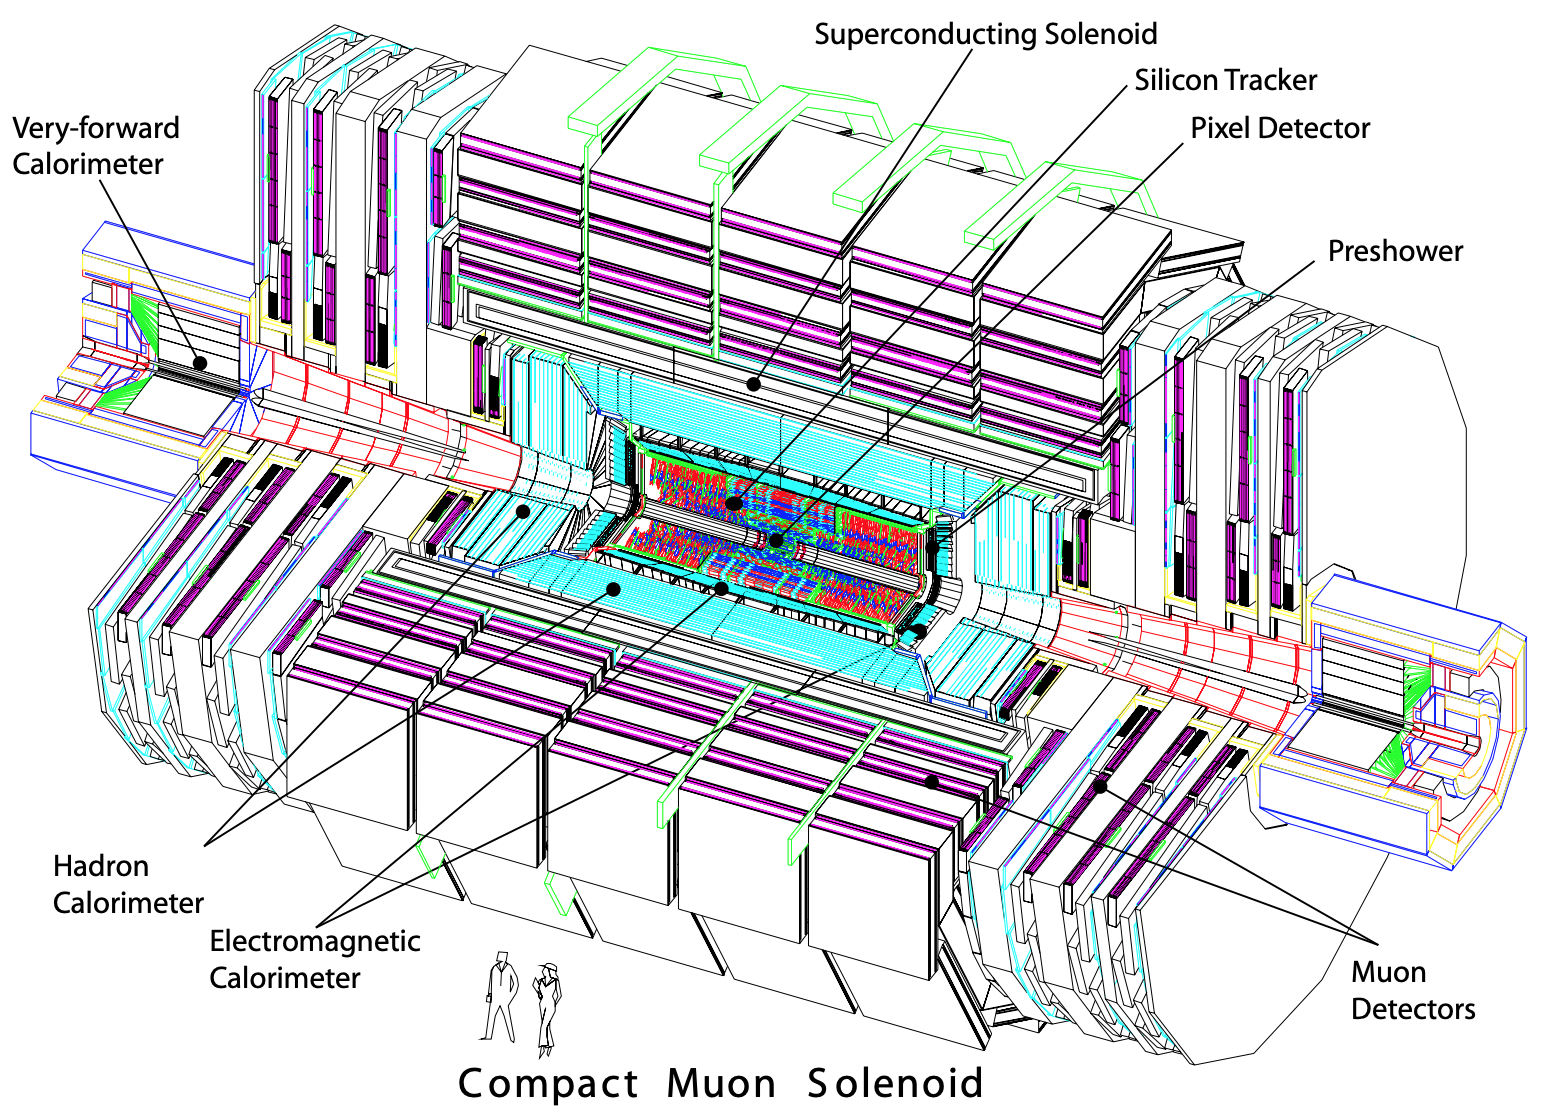
\includegraphics[width=0.8\linewidth]{figures/cms/cms_detector_schematic.png}
    \caption{Schematic of the various components of the CMS detector. Taken from~\cite{Chatrchyan:2008aa}.}
    \label{fig:cms_schematic}
\end{figure}

As its name suggests, the primary feature of the CMS detector is a superconducting solenoid providing a magnetic field of 4~T.
The purpose of the magnetic field is to bend the path of charged particles originating from inelastic proton-proton interactions: the precise spatial resolution of the tracker and muon system allows one to determine a particle's radius of curvature, in turn allowing one to determine the particle's momentum.
Excellent momentum resolution of charged particles supports nearly every physics analysis performed with the CMS detector, but is especially important for determining the invariant mass of heavy resonances (e.g. studying the properties of the Higgs boson in the H $\to$ ZZ$^{*} \to 4l$ channel), distinguishing between hadronic jets which originate from b quarks from those which originate from gluons or light-flavor quarks (e.g. the H $\to$ bb decay channel and searches for new physics involving final states with b-jets), and for precise resolution of the missing transverse energy (e.g. final states with neutrinos or searches for new physics involving final states with undetected dark matter or supersymmetry candidate particles).

The other major components of the detector include: 
\begin{itemize}
    \item The tracker, which allows for identification and excellent momentum resolution of charged particles.
    \item The electromagnetic calorimeter (ECAL), which allows for identification of electrons and photons, particularly important for H $\to \gamma \gamma$ physics.
    \item The hadronic calorimeter (HCAL), which assists in the identification and momentum resolution of charged hadrons and provides the only handle on measuring neutral hadrons.
    \item The muon system, which enables better momentum resolution of very high energy ($\mathcal O$(TeV)) muons (while the tracker excels in providing good momentum resolution for lower energy, $\mathcal O$(GeV) muons).
\end{itemize}
Each of these components is described in greater detail in the following subsections.

A design consideration common to multiple subdetector components is the goal of hermeticity: a fully hermetic detector is able to measure particles emerging in any direction from an inelatic collision.
In other words, a hermetic detector has full coverage of the $4\pi$ steradians of solid angle surrounding the interaction point.
The CMS detector is not fully hermetic, as it is practically impossible to measure particles which emerge parallel to the LHC's proton beams.
Still, the CMS detector is able to measure very forward particles (with ``forward'' meaning ``close to parallel with the beam axis''), aiding the nearly complete reconstruction of the final state of a given pp interaction, which is essential for resolution of the missing transverse energy.

To expand upon the concepts of hermeticity and the identification of forward particles, we must first introduce the coordinate system used to describe the CMS detector.
Given the cylindrical shape of the detector, standard cylincdrical coordinates form the basis of the coordinate system: the $\hat{z}$-axis is defined as the axis along which the proton beams travel, and the $\hat{\phi}$ direction then coincides with the detector's circular symmetry perpendicular to the beam axis.
Instead of the typical polar angle $\hat{\theta}$, position is usually expressed in terms of pseudorapidity, defined in terms of $\theta$ as
\begin{equation}
    \eta = -\ln \Bigg[ \tan \bigg(\frac{\theta}{2}\bigg) \Bigg].
\end{equation}
A pseudorapidity of $\eta = 0$ corresponds to a direction perpendicular to the beam axis, while $\eta = \infty$ corresponds to a direction parallel to the beam axis.
Pseudorapidity is convenient for a number of reasons, including the fact that it is nearly Lorentz invariant under boosts along the $\hat{z}$-axis.
We say that it is ``nearly'' Lorentz invariant as this is only true for massless particles.
However, at the LHC, the transverse momentum of a given particle is typically sufficiently larger than the mass ($\pT >> m$) such that the pseudorapidity is approximately Lorentz invariant. 

Much of the reason for CMS's 20m of length in the direction of the beam axis is motivated by the goal of hermeticity.
The forward calorimeter (described in greater detail in Sec.~\ref{sec:cms_hcal}) provides coverage up to pseudorapidities of $|\eta| \leq 5.0$.
Pairing the extensive range in pseudorapidities with the CMS detector's complete coverage in the $\hat{\phi}$-direction, the CMS detector is nearly hermetic, aiding the resolution of missing transverse energy and consequently the ability to infer the presence of undetected particles.
The exact coverage of each of the detector subcomponents is discussed in greater detail in the following subsections.

\subsection{Solenoid}
The solenoid installed in the CMS detector is over 12m in length and 6m in diameter, capable of providing a 4~T magnetic field.
The purpose of such a strong magnetic field is to bend the trajectories of charged particles (as illustrated in Fig.~\ref{fig:cms_transverse_view}, allowing CMS to measure their momentum, mass, and charge.
Fig.~\ref{fig:cms_transverse_view} depicts the three major classes of particles which have their trajectories curved by the magnetic field produced by the solenoid: an electron (red), a charged hadron (green), and a muon (blue).
Measurements of the momenta of electrons are also aided by the ECAL (described in Sec.~\ref{sec:cms_ecal}), those of charged hadrons are also aided by the HCAL (described in Sec.~\ref{sec:cms_hcal}), and those of muons are also aided by the muon system (described in Sec.~\ref{sec:cms_muon_system}).

\begin{figure} [htbp!]
    \centering
    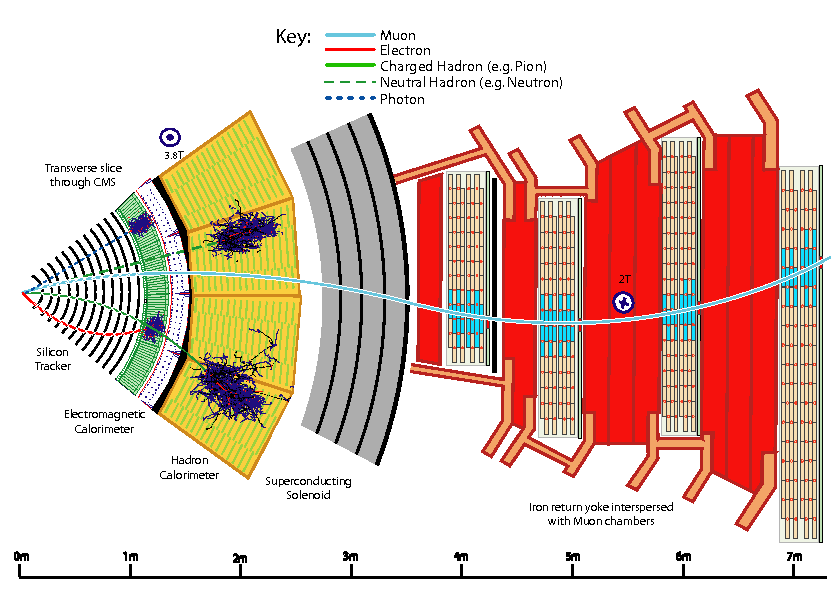
\includegraphics[width=\linewidth]{figures/cms/cms_transverse_view.png}
    \caption{Depiction of a transverse slice of the CMS detector, along with trajectories of particles of different types. Taken from~\cite{Sirunyan:2270046}.}
    \label{fig:cms_transverse_view}
\end{figure}

The solenoid is installed around the the tracker (Sec.~\ref{sec:cms_tracker}), the ECAL (Sec.~\ref{sec:cms_ecal}), and the HCAL (Sec.~\ref{sec:cms_hcal}) which is why the solenoid must be so large.
In order to support the massive current (over $10^4$~A) required for the magnetic field, the solenoid is constructed with superconducting Niobium-Titanium (NbTi), and its temperature must be kept sufficiently low to ensure superconductivity of the NbTi. 

\subsection{Tracker} \label{sec:cms_tracker}
The innermost component of the CMS detector is the silicon tracker, and its primary aim is to provide the precise reconstruction of charged particles and secondary vertices (an inelastic pp collision is deemed a ``primary vertex'' while decays of particles produced from a primary vertex are deemed ``secondary vertices'').
The tracker is nearly 6~m in length and 2.5m in diameter, composed of an inner pixel detector with three layers ranging from 4-10~cm and an outer silicon strip tracker with ten layers ranging to 1.1~m.
Both the pixel detector and the silicon strip tracker are accompanied by endcap disks on either end of the barrel, extending the pseudorapidity coverage to $|\eta| \leq 2.5$.
Between the data-taking periods corresponding to 2016 and 2017, the inner pixel detector was upgraded~\cite{Botta:2285433}, extending the coverage of the tracker up to $|\eta| \leq 3.0$.
As shown in Fig.~\ref{fig:cms_tracker_upgrade}, the number of fake tracks, the impact parameter resolution, and the vertex resolution are each improved as well, resulting in an approximately 10\% improvement in the b-tagging efficiency for a fixed fake rate.

\begin{figure} [htbp!]
    \centering
    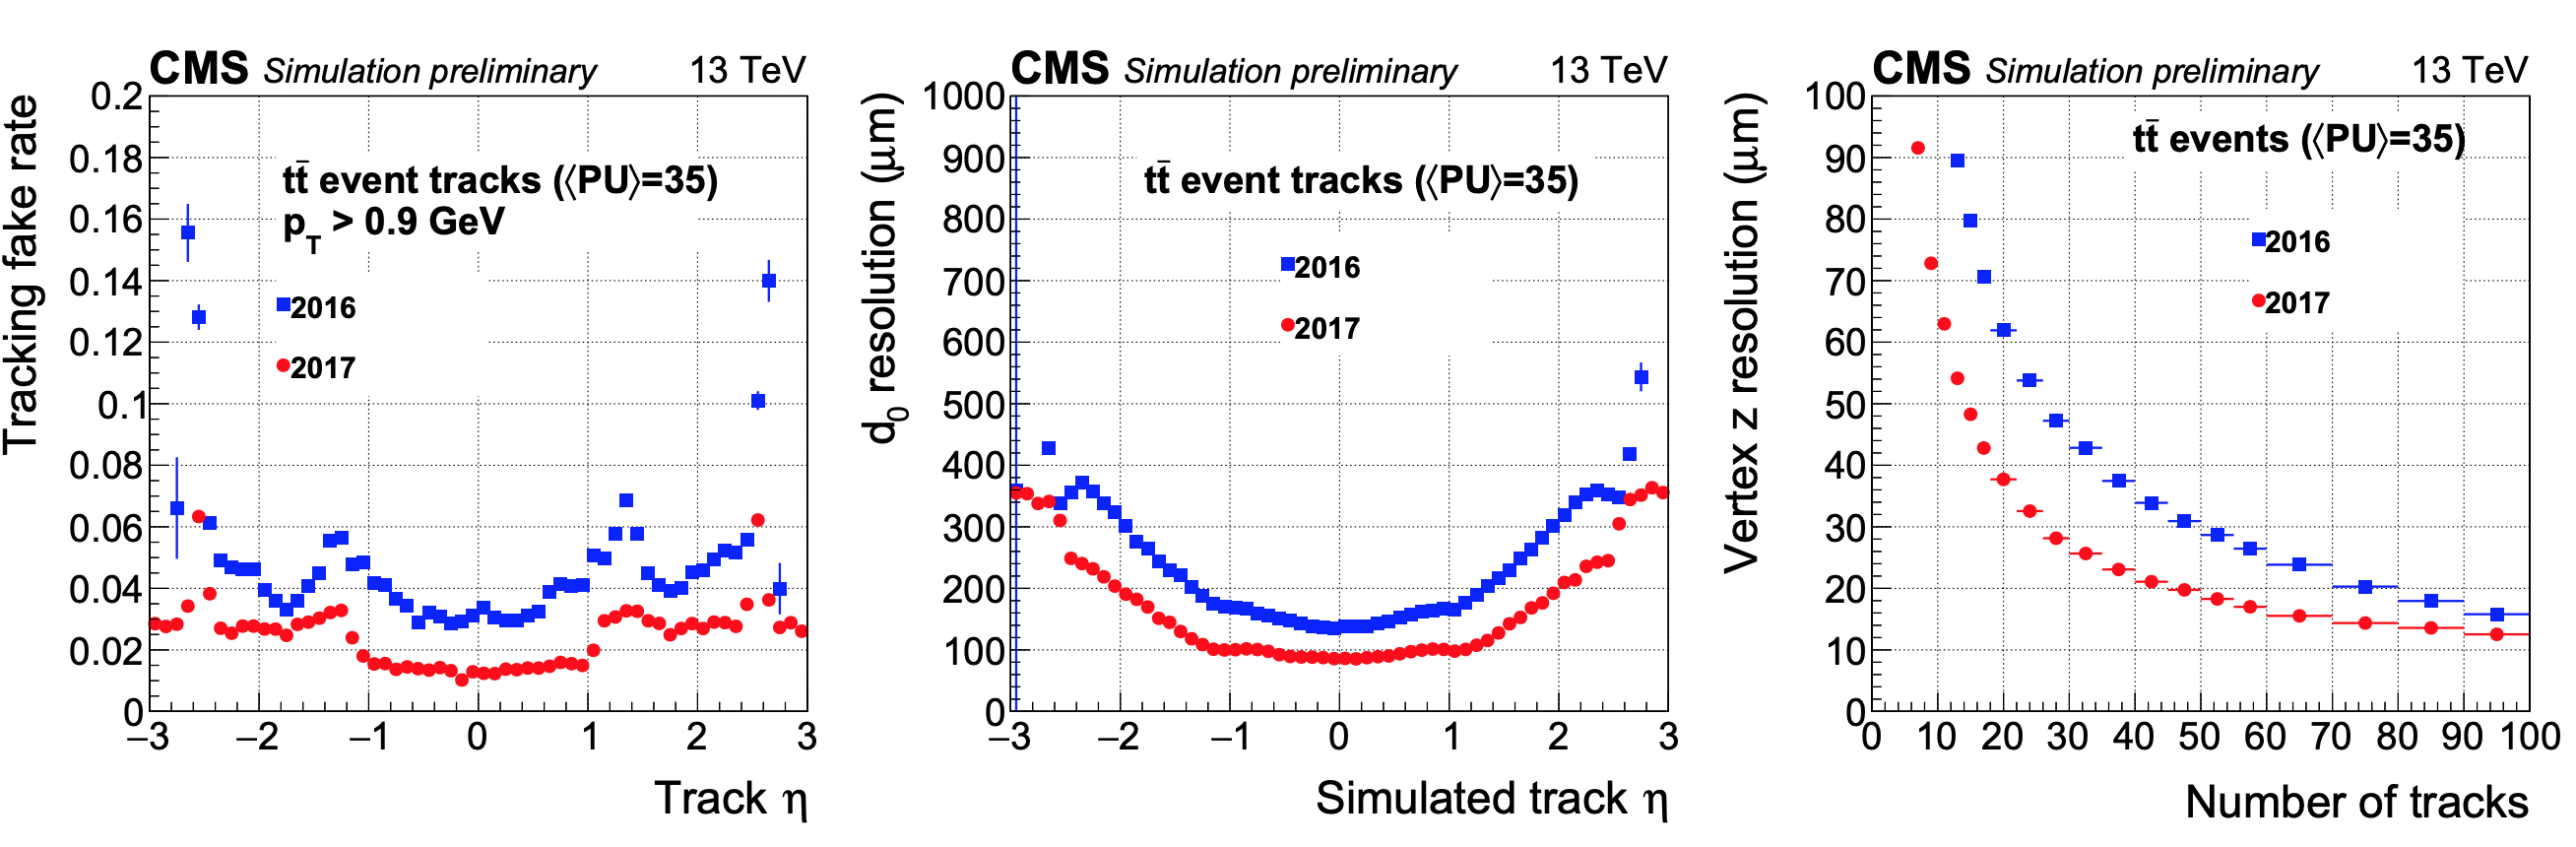
\includegraphics[width=\linewidth]{figures/cms/cms_pixel_upgrade.png}
    \caption{Comparison of tracker performance before and after the upgrade to the pixel detector, performed in between the 2016 and 2017 data-taking periods. Taken from~\cite{Botta:2285433}.}
    \label{fig:cms_tracker_upgrade}
\end{figure}

The primary design considerations for the tracker include the following:
\begin{itemize}
    \item Ability to reconstruct a large number of charged particles in each bunch crossing, with $\mathcal O(1000)$ charged particles expected from a single bunch crossing at the LHC design luminosity of $\mathcal L = 1034$~cm$^{-2}$~s$^{-1}$ (corresponding to about 20 individual pp interactions).
    \item Ability to reconstruct charged particles with precise temporal resolution, with bunch crossings separated by a distance corresponding to 25~ns.
    \item Minimal interaction of photons with the tracker material, as precise measurements of photons are vital to studying Higgs physics in the \Hgg decay channel.
\end{itemize}

The first two considerations are in direct conflict with the third consideration: a tracker with high granularity and fast response implies large power density of electronics, which requires efficient cooling. This increases the material budget of the tracker, increasing the chances of bremsstrahlung and photon conversions, which in turn degrade the ECAl's photon energy resolution. 
An acceptable compromise providing both execllent tracking and excellent photon resolution was achieved with the tracker design depicted in Fig.~\ref{fig:cms_tracker_schematic}.

\begin{figure} [htbp!]
    \centering
    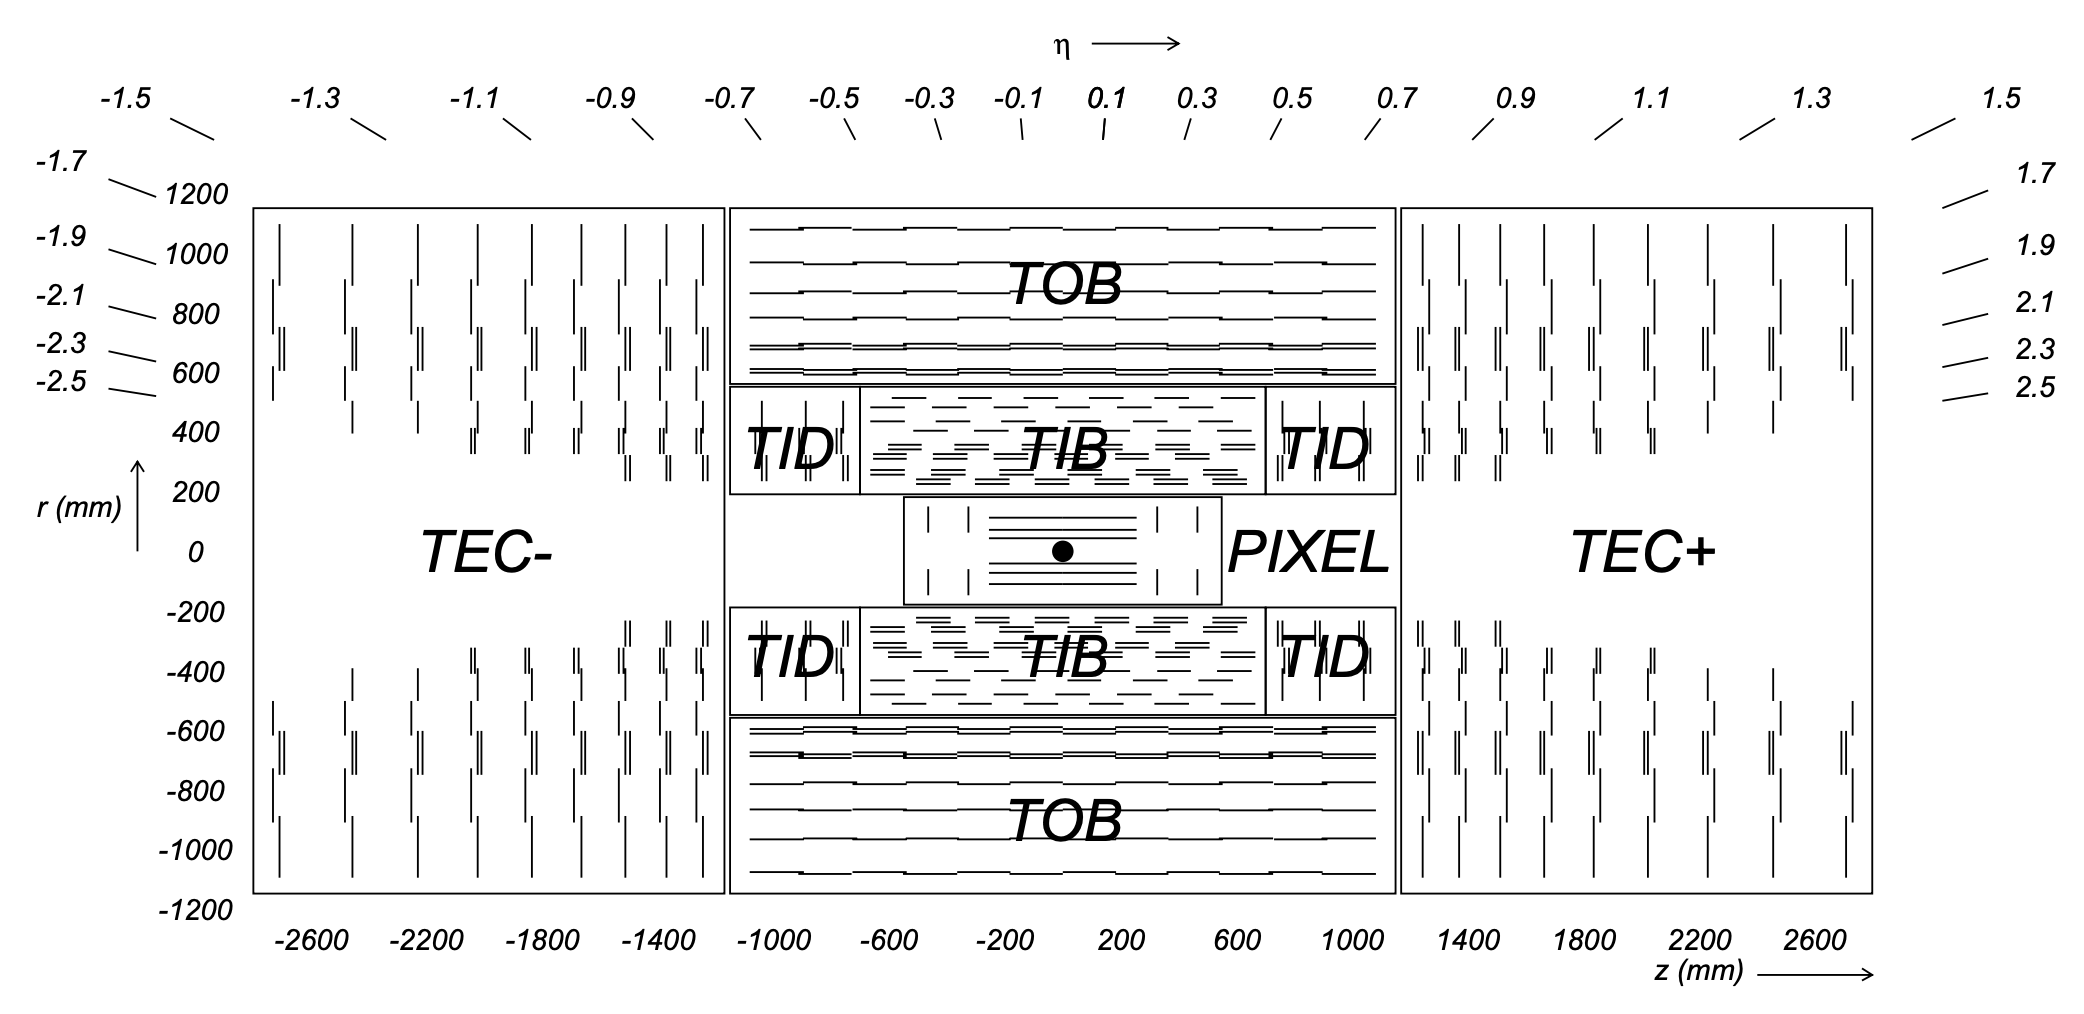
\includegraphics[width=0.8\linewidth]{figures/cms/cms_tracker_schematic.png}
    \caption{Schematic of the CMS tracker from a cross-sectional viewpoint. TIB, TOB, TID, and TEC represent the tracker inner barrel, tracker outer barrel, tracker inner disk, and tracker endcap components, respectively. Taken from~\cite{Chatrchyan:2008aa}.}
    \label{fig:cms_tracker_schematic}
\end{figure}

The material budget for the CMS tracker is shown in Fig.~\ref{fig:cms_tracker_budget}, showing the thickness of the tracker material in terms of the characteristic radiation lengths $X_0$ (for electromagnetic particles, e.g. electrons and photons) and characteristic nuclear interaction lengths $\lambda_I$ (i.e. for hadrons).
The tracker thickness in terms of both radiation lengths and nuclear interaction lengths is lowest in the most central part of the barrel and increases in the more forward components, accounting for one of the reasons that CMS achieves better energy resolution for very central particles.

\begin{figure} [htbp!]
    \centering
    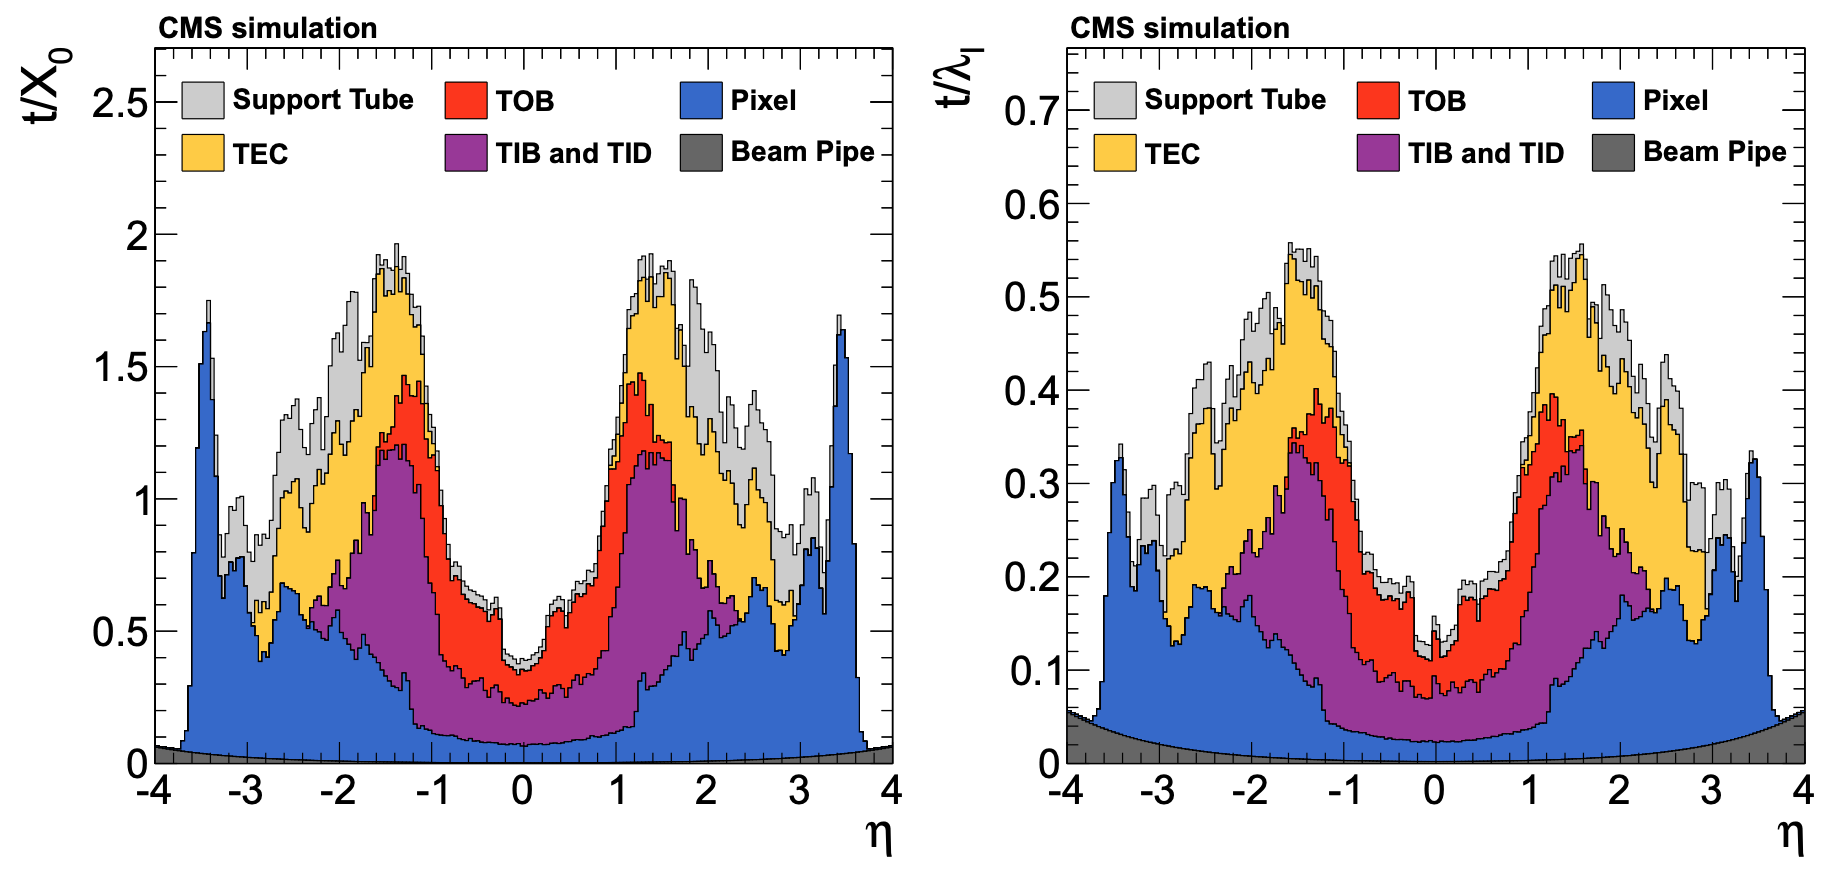
\includegraphics[width=\linewidth]{figures/cms/cms_tracker_budget.png}
    \caption{The material budget for the CMS tracker shown for both the characteristic radiation lengths of electromagnetic interactions (left) and the characteristic nuclear interaction lengths of hadronic interactions (right), with the contributions of each of the tracker subcomponents shown individually. Taken from~\cite{Chatrchyan:1704291}.}
    \label{fig:cms_tracker_budget}
\end{figure}

The tracking effieciency achieved by the CMS tracker is shown in Fig.~\ref{fig:cms_tracker_eff}, for muons, pions, and electrons as a function of their transverse momentum.
In general, the tracker achieves higher efficiency for muons than for electrons or pions, as electrons are more likely to emit radiation via bremsstrahlung and charged pions may undergo nuclear interactions with the tracker material.
Energy resolution of high \pT ($\mathcal O(TeV)$) muons is assisted by the muon system, as shown in Fig.~\ref{fig:cms_muon_vs_tracker}.

\begin{figure} [htbp!]
    \centering
    \begin{tabular}{c c c}
        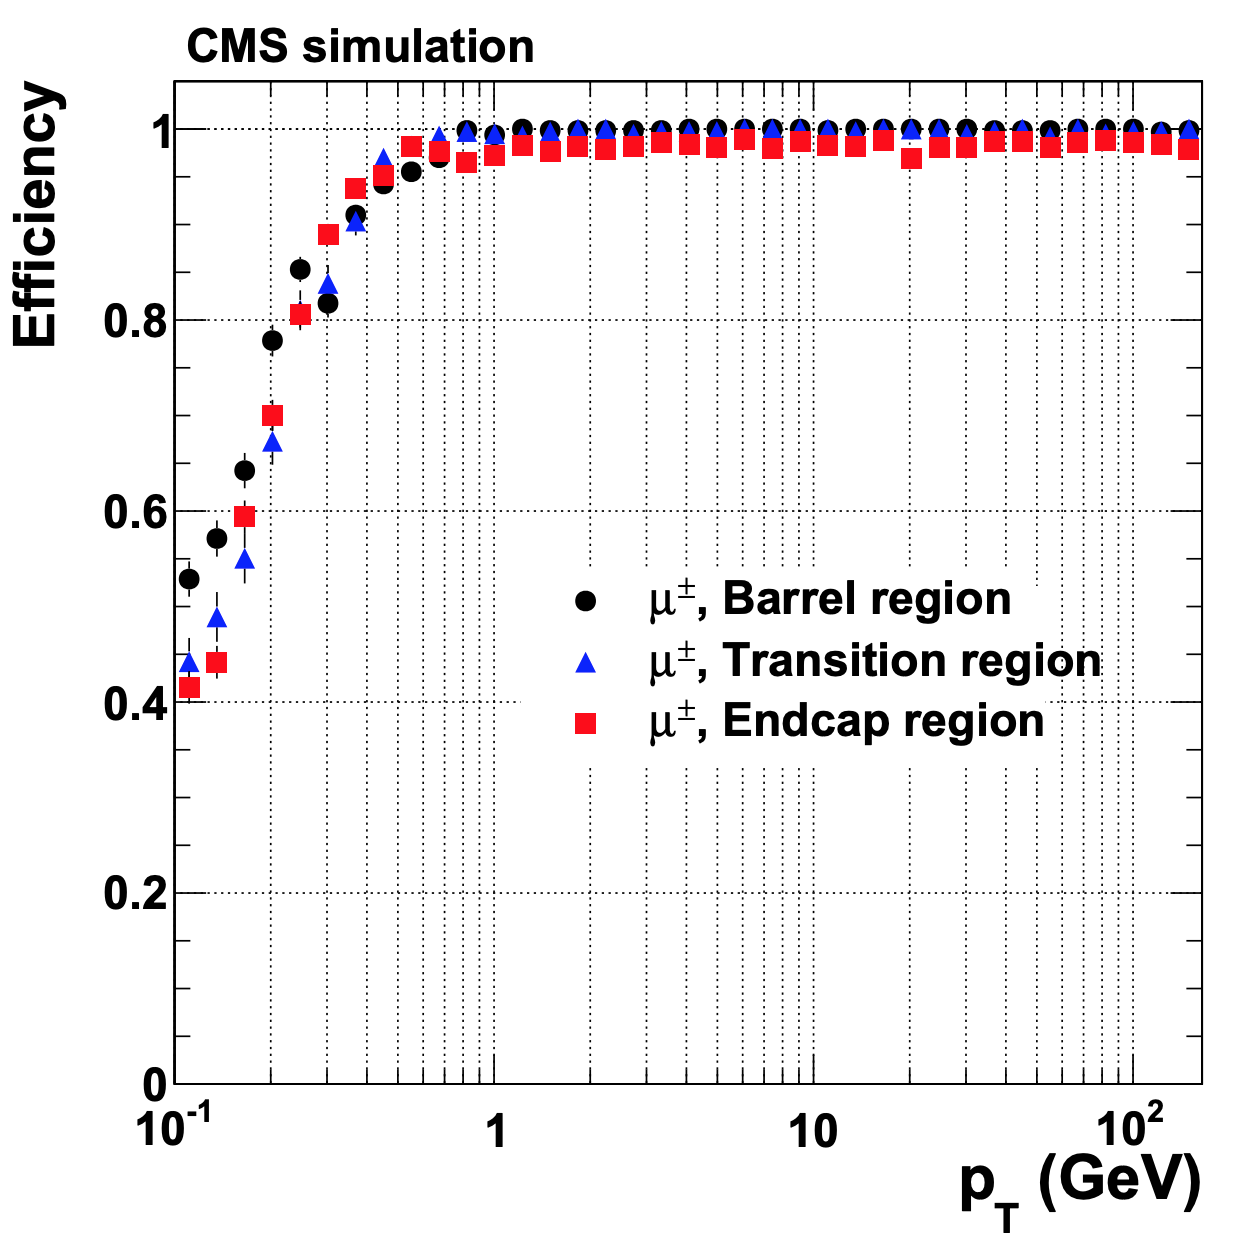
\includegraphics[width=0.33\linewidth]{figures/cms/cms_tracker_muon.png} &
        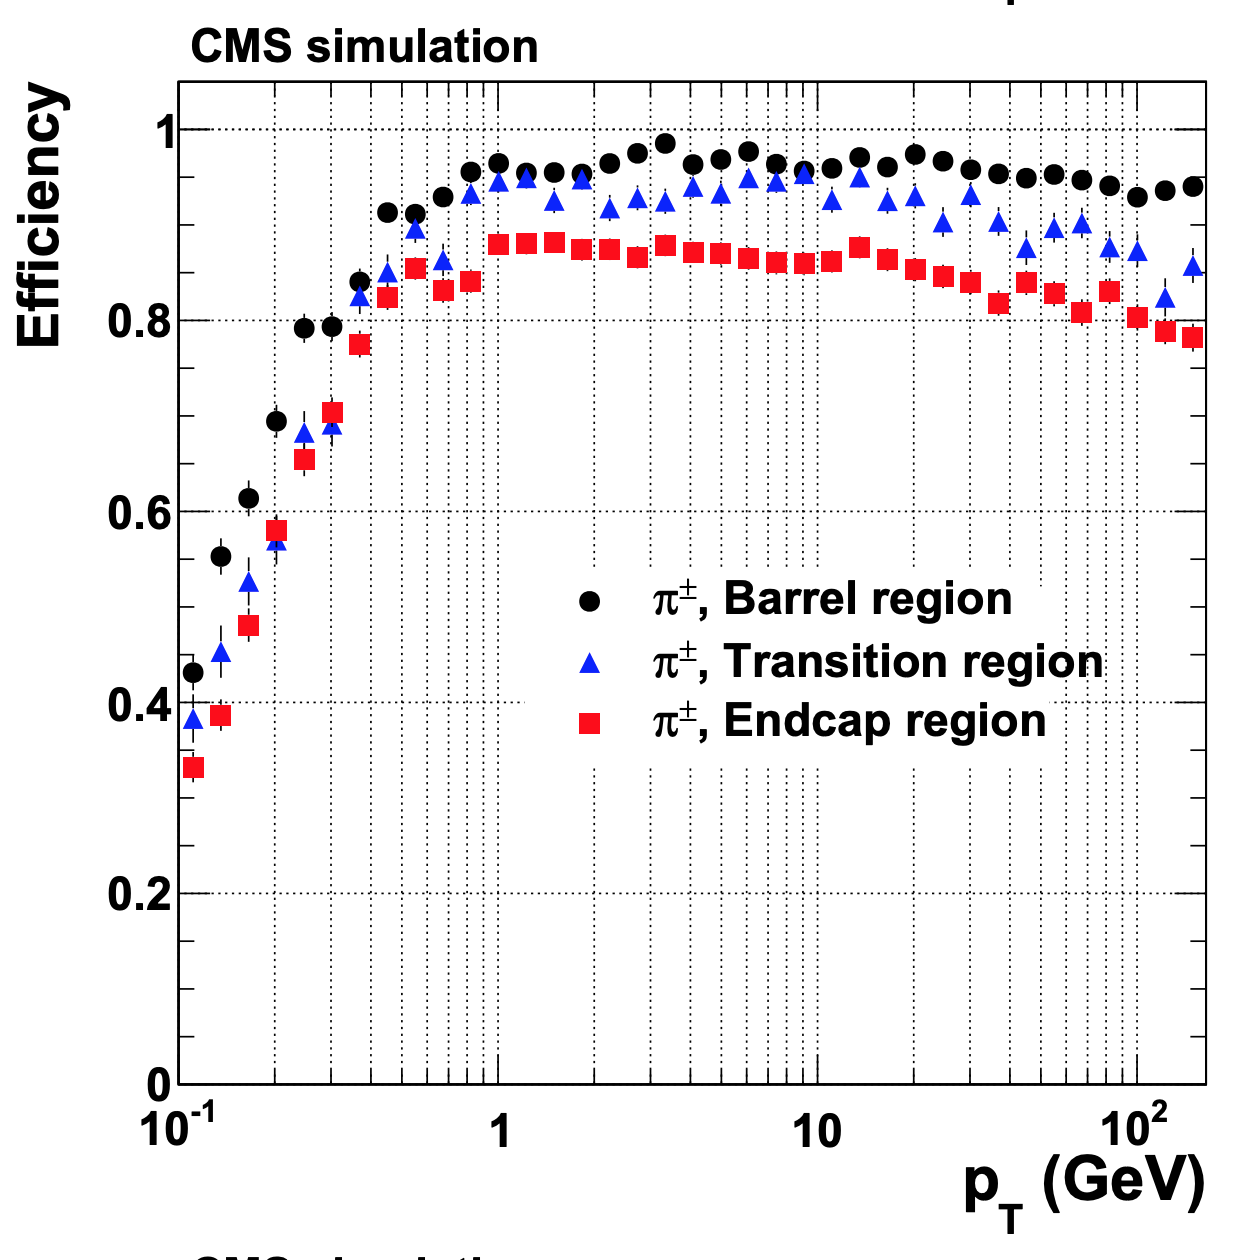
\includegraphics[width=0.33\linewidth]{figures/cms/cms_tracker_pion.png} &
        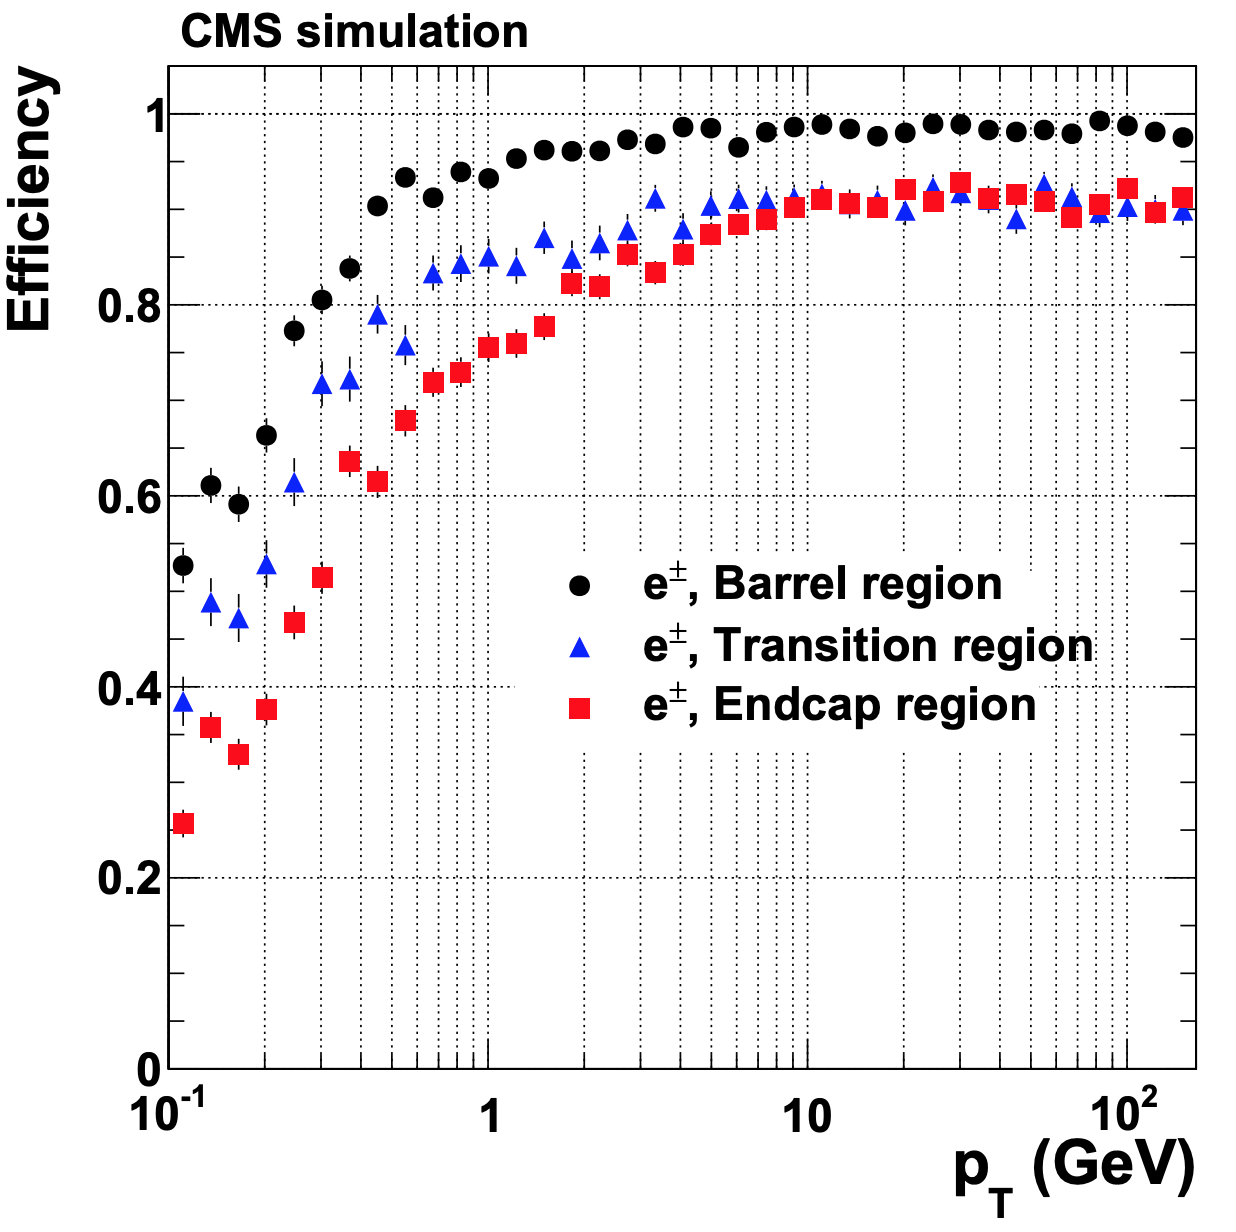
\includegraphics[width=0.33\linewidth]{figures/cms/cms_tracker_electron.png}
    \end{tabular}
    \caption{Tracking efficiency as a function of \pT for muons (left), charged pions (middle), and electrons (right), shown separately for the barrel (black), transition region (blue), and endcap (red). Taken from~\cite{Chatrchyan:1704291}.}
    \label{fig:cms_tracker_eff}
\end{figure}


\subsection{Electromagnetic Calorimeter} \label{sec:cms_ecal}

\subsection{Hadronic Calorimeter} \label{sec:cms_hcal}

\subsection{Muon System} \label{sec:cms_muon_system}

\begin{figure} [htbp!]
    \centering
    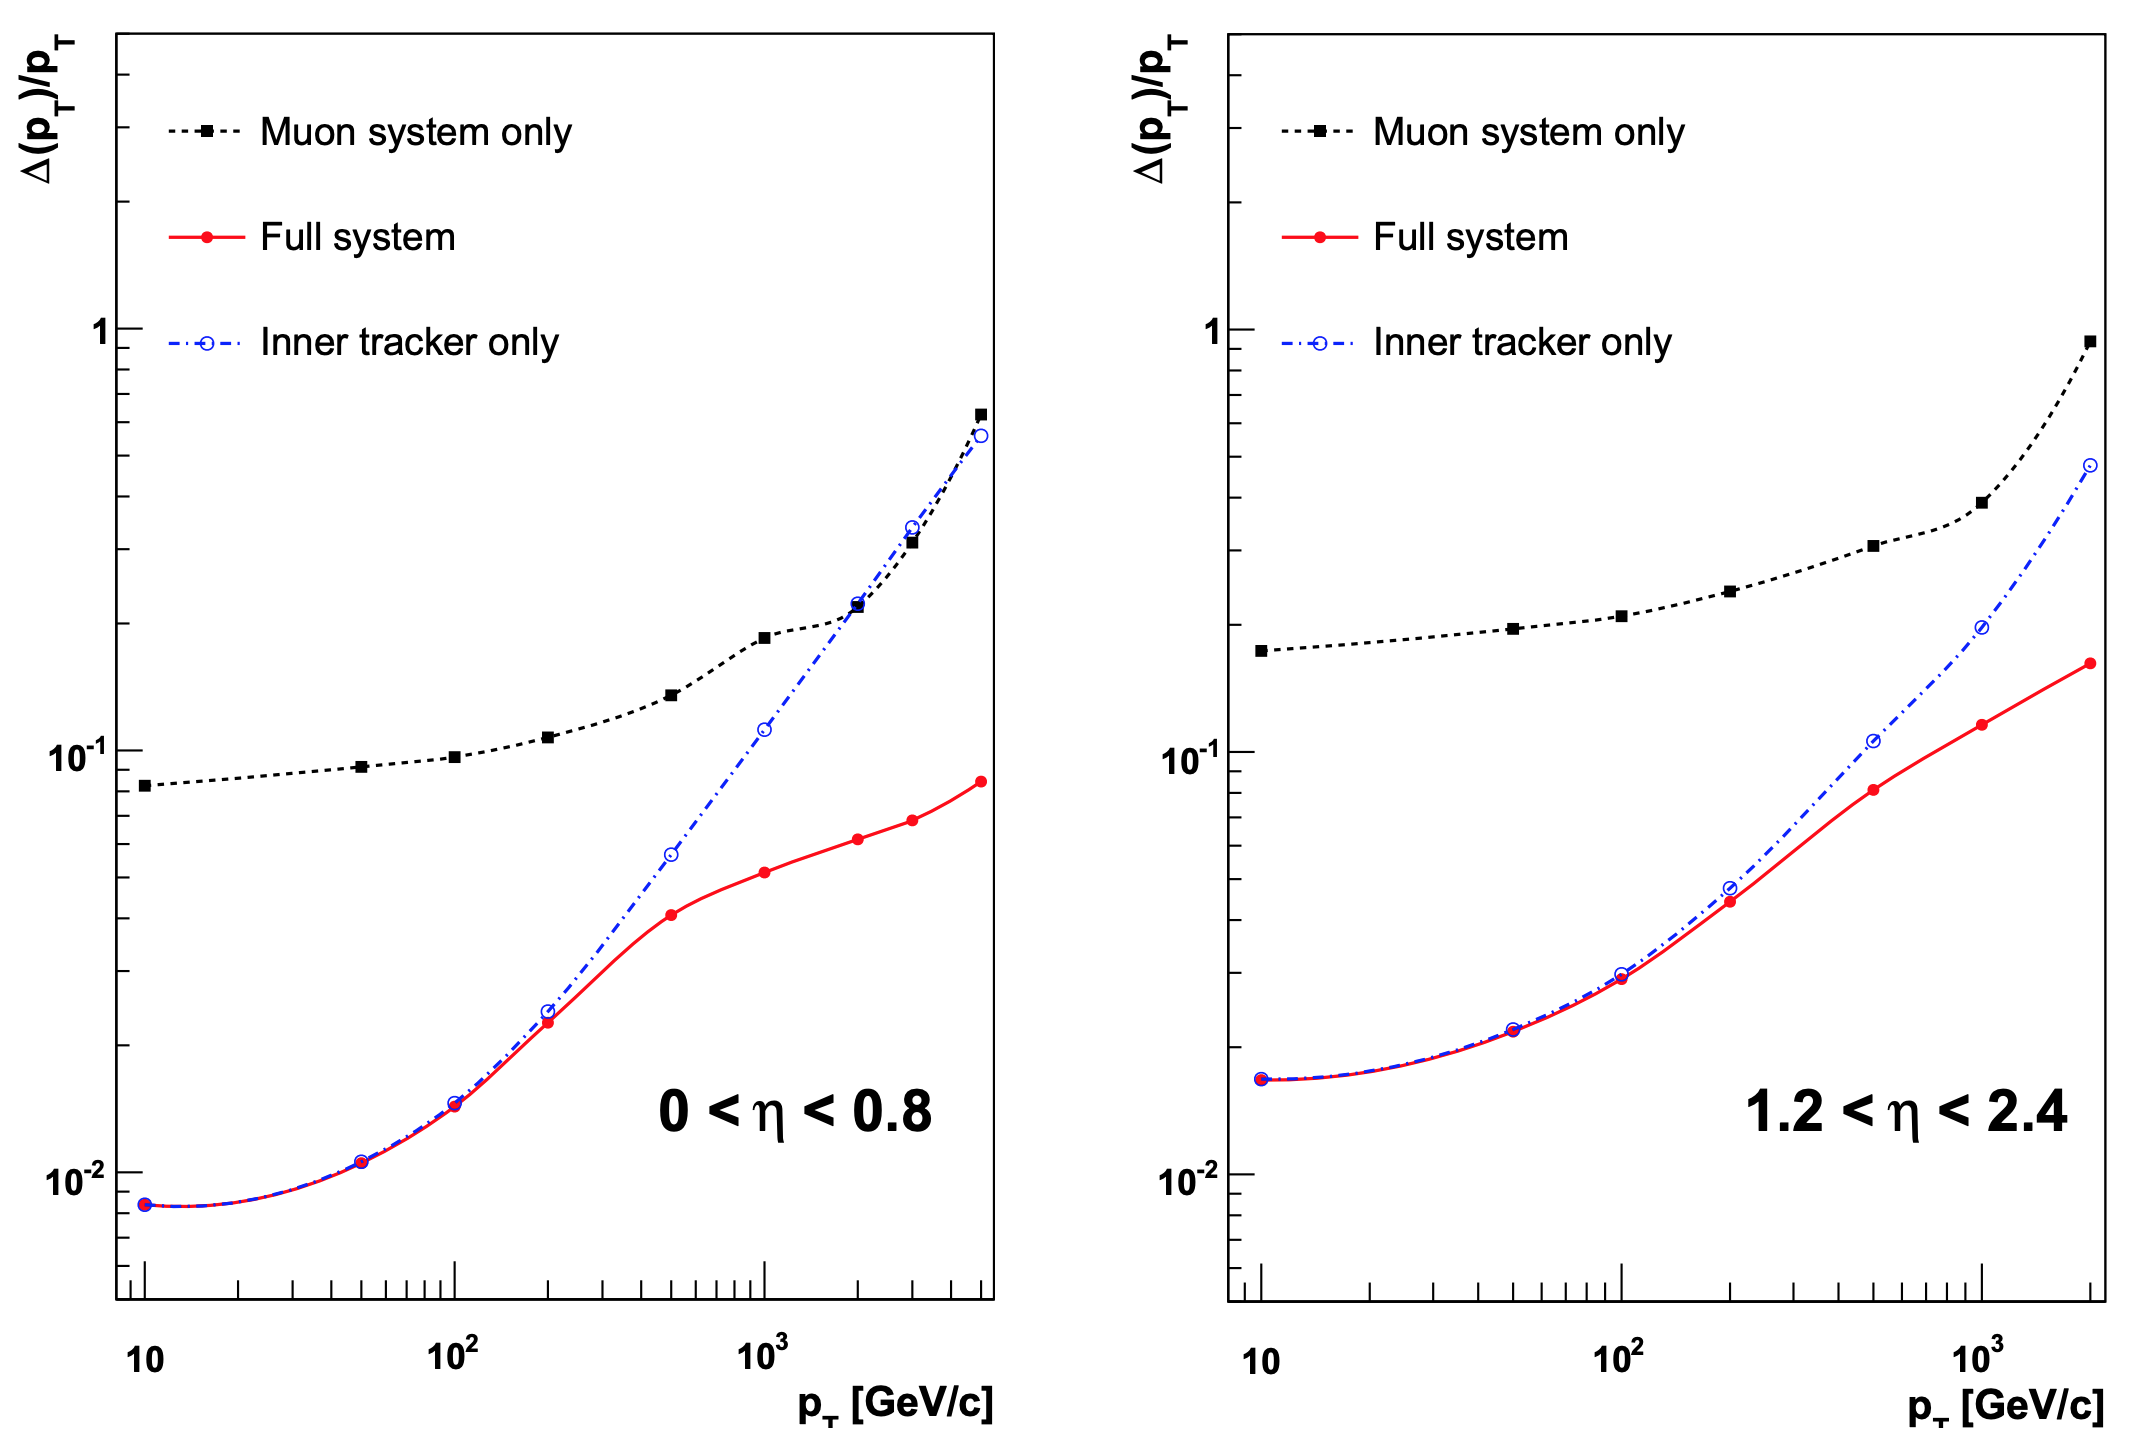
\includegraphics[width=0.8\linewidth]{figures/cms/cms_tracker_vs_muon.png}
    \caption{Fractional momentum resolution for muons reconstructed by the CMS detector, shown for reconstructions using the inner tracker only (blue), the muon system only (black), and the combination of measurements from both subdetectors (red). The muon system improves significantly the momentum resolution of $\mathcal O$(TeV) muons. Taken from~\cite{Chatrchyan:2008aa}.}
    \label{fig:cms_muon_vs_tracker}
\end{figure}

\subsection{Trigger System} \label{sec:cms_trigger}

\subsubsection{L1 Trigger}

\subsubsection{HLT Trigger}
